\documentclass[12pt]{article}\usepackage[]{graphicx}\usepackage[]{color}
%% maxwidth is the original width if it is less than linewidth
%% otherwise use linewidth (to make sure the graphics do not exceed the margin)
\makeatletter
\def\maxwidth{ %
  \ifdim\Gin@nat@width>\linewidth
    \linewidth
  \else
    \Gin@nat@width
  \fi
}
\makeatother

\definecolor{fgcolor}{rgb}{0.345, 0.345, 0.345}
\newcommand{\hlnum}[1]{\textcolor[rgb]{0.686,0.059,0.569}{#1}}%
\newcommand{\hlstr}[1]{\textcolor[rgb]{0.192,0.494,0.8}{#1}}%
\newcommand{\hlcom}[1]{\textcolor[rgb]{0.678,0.584,0.686}{\textit{#1}}}%
\newcommand{\hlopt}[1]{\textcolor[rgb]{0,0,0}{#1}}%
\newcommand{\hlstd}[1]{\textcolor[rgb]{0.345,0.345,0.345}{#1}}%
\newcommand{\hlkwa}[1]{\textcolor[rgb]{0.161,0.373,0.58}{\textbf{#1}}}%
\newcommand{\hlkwb}[1]{\textcolor[rgb]{0.69,0.353,0.396}{#1}}%
\newcommand{\hlkwc}[1]{\textcolor[rgb]{0.333,0.667,0.333}{#1}}%
\newcommand{\hlkwd}[1]{\textcolor[rgb]{0.737,0.353,0.396}{\textbf{#1}}}%

\usepackage{framed}
\makeatletter
\newenvironment{kframe}{%
 \def\at@end@of@kframe{}%
 \ifinner\ifhmode%
  \def\at@end@of@kframe{\end{minipage}}%
  \begin{minipage}{\columnwidth}%
 \fi\fi%
 \def\FrameCommand##1{\hskip\@totalleftmargin \hskip-\fboxsep
 \colorbox{shadecolor}{##1}\hskip-\fboxsep
     % There is no \\@totalrightmargin, so:
     \hskip-\linewidth \hskip-\@totalleftmargin \hskip\columnwidth}%
 \MakeFramed {\advance\hsize-\width
   \@totalleftmargin\z@ \linewidth\hsize
   \@setminipage}}%
 {\par\unskip\endMakeFramed%
 \at@end@of@kframe}
\makeatother

\definecolor{shadecolor}{rgb}{.97, .97, .97}
\definecolor{messagecolor}{rgb}{0, 0, 0}
\definecolor{warningcolor}{rgb}{1, 0, 1}
\definecolor{errorcolor}{rgb}{1, 0, 0}
\newenvironment{knitrout}{}{} % an empty environment to be redefined in TeX

\usepackage{alltt} % JASA requires 12 pt font for manuscripts

\usepackage{afterpage} % for better control of the floats

%\usepackage{endfloat} % just for while I am writing

% for citations
\usepackage[authoryear]{natbib} % natbib required for JASA
% \usepackage[colorlinks=true, citecolor=blue, linkcolor=blue]{hyperref} % comment out and use url package for submission

% for the fancy tables with the icons
%\usepackage[margin=1.0in]{geometry}% http://ctan.org/pkg/margin
\usepackage{booktabs}% http://ctan.org/pkg/booktabs
\usepackage{array}% http://ctan.org/pkg/array
\newcolumntype{M}{>{\centering\arraybackslash}m{\dimexpr.05\linewidth-2\tabcolsep}}



\usepackage[usenames,dvipsnames]{xcolor}


%\definecolor{Blue}{rgb}{0,0,0.5}
\newcommand{\hh}[1]{{\color{magenta} #1}}
\newcommand{\al}[1]{{\color{ForestGreen} #1}}

\newcolumntype{C}[1]{>{\centering}m{#1}}
% fonts
%\usepackage{kpfonts}

% for figures
\usepackage{graphicx,psfrag,epsf}
\usepackage{enumerate}
\usepackage{natbib}
\usepackage{url} % not crucial - just used below for the URL 

\graphicspath{{figure/}}


%\pdfminorversion=4
% NOTE: To produce blinded version, replace "0" with "1" below.
\newcommand{\blind}{0}

% DON'T change margins - should be 1 inch all around.
\addtolength{\oddsidemargin}{-.5in}%
\addtolength{\evensidemargin}{-.5in}%
\addtolength{\textwidth}{1in}%
\addtolength{\textheight}{1.3in}%
\addtolength{\topmargin}{-.8in}%


\usepackage{wrapfig,float}
\usepackage{caption}
\usepackage{subcaption}

% help with editing and coauthoring
\usepackage{todonotes}
\newcommand{\alnote}[1]{\todo[inline,color=green!40]{#1}}
\newcommand{\hhnote}[1]{\todo[inline,color=magenta!40]{#1}}

% For math typsetting
\usepackage{bm}
\usepackage{amstext}
\usepackage{amssymb}
\usepackage{amsmath}
\usepackage{amsfonts}
\usepackage{multirow}

% A few commands to make typing less tedious
\newcommand{\inv}{\ensuremath{^{-1}}}
\newcommand{\ginv}{\ensuremath{^{-}}}
\newcommand{\trans}{\ensuremath{^\prime}}
\newcommand{\E}{\ensuremath{\mathrm{E}}}
\newcommand{\var}{\ensuremath{\mathrm{Var}}}
\newcommand{\cov}{\ensuremath{\mathrm{Cov}}}


% \title{Variations of Q-Q Plots -- the Power of our Eyes!}
% 
% \author{Adam Loy, Lendie Follett, Heike Hofmann
% \thanks{Adam Loy is an Assistant Professor in the Department of Mathematics, Lawrence University, Appleton, WI, 54911 (e-mail: adam.m.loy@lawrence.edu);  Lendie Follett is a Ph.D. student in the Department of Statistics and Statistical Laboratory, Iowa State University, Ames, IA 50011-1210; Heike Hofmann is a Professor in the Department of Statistics and Statistical Laboratory, Iowa State University, Ames, IA 50011-1210. This work was funded in part by National Science Foundation grant DMS 1007697. All data  in the study was collected  with approval from the internal review board IRB 10-347.}}
\IfFileExists{upquote.sty}{\usepackage{upquote}}{}
\begin{document}

\def\spacingset#1{\renewcommand{\baselinestretch}%
{#1}\small\normalsize} \spacingset{1}


\if0\blind
{
  \title{\bf Variations of Q-Q Plots -- the Power of our Eyes!}
\author{Adam Loy, Lendie Follett, Heike Hofmann
\thanks{Adam Loy is an Assistant Professor in the Department of Mathematics, Lawrence University, Appleton, WI, 54911 (e-mail: adam.m.loy@lawrence.edu);  Lendie Follett is a Ph.D. student in the Department of Statistics and Statistical Laboratory, Iowa State University, Ames, IA 50011-1210; Heike Hofmann is a Professor in the Department of Statistics and Statistical Laboratory, Iowa State University, Ames, IA 50011-1210. This work was funded in part by National Science Foundation grant DMS 1007697. All data  in the study was collected  with approval from the internal review board IRB 10-347.}}
  \maketitle
} \fi

\if1\blind
{
  \bigskip
  \bigskip
  \bigskip
  \begin{center}
    {\LARGE\bf Variations of Q-Q Plots -- the Power of our Eyes!}
\end{center}
  \medskip
} \fi


\bigskip

\begin{abstract}
In statistical modeling we strive to specify models that resemble data collected in studies or observed from processes. Consequently, distributional specification and parameter estimation are central to parametric models. Graphical procedures, such as the quantile-quantile (Q-Q) plot, are arguably the most widely used method of distributional assessment, though critics find their interpretation to be overly subjective. Formal goodness-of-fit tests are available and are quite powerful, but only indicate whether there is a lack of fit, not why there is lack of fit. In this paper we explore the use of the lineup protocol to inject rigor to graphical distributional assessment and compare its power to that of formal distributional tests. We find that lineups of standard Q-Q plots are more powerful than lineups of de-trended Q-Q plots and that lineup tests are more powerful than traditional tests of normality. While we focus on diagnosing non-normality, our approach is general and can be directly extended to the assessment of other distributions.
% 
% 
% this paper holds two messages: 
% a) our eyes are well suited to assess distributional assumptions. We  objectively measure  power and sensitivity of Q-Q plots using lineup tests. 
% At the example of normal distributions we can show that Q-Q plots are better at identifying non-normality than some prominent tests of normality, such as Shapiro-Wilks,  Anderson-Darling,  Kolmogorov-Smirnov, Lilliefors, or  Cramer-von-Mises.
% 
% b) Out of the variations discussed, de-trended Q-Q plots perform significantly worse than the other two variants. This is surprising, because cognitive theory tells us, that de-trended plots should be better suited in assessing the difference between empirical and hypothesized  distribution.
% \keywords{Quantile-Quantile plot, Normality test, Statistical graphics, Lineup protocol, Visual inference}
\end{abstract}

{\it Keywords:} Quantile-Quantile plot; Normality test; Statistical graphics; Lineup protocol; Visual inference
\clearpage
\spacingset{1.45}









%------------------------------------------------------------------------------------
\section{Introduction}
%------------------------------------------------------------------------------------

In statistical modeling we strive to specify models that resemble data collected in studies or observed from processes. Consequently, %could generate the observed data. 
distributional specification and parameter estimation are central to parametric models.
%Parametric models center around the specification of a family of probability distributions and the estimation of the parameters such that the estimated distribution could have pluasibly generated the data. 
The statistical modeling process is cyclical \citep{tukey:eda}, so after parameters are estimated and the model is checked, the process might continue through another cycle with a refined model formulation. Model checking is central to statistical modeling; in particular, any conclusions based on a model depend  on  correct distributional specifications. For example, prediction intervals in the classical regression setting depend directly on the assumption of normality, so they are quite sensitive to departures from normality. 

Graphical procedures, such as the quantile-quantile (Q-Q) plot \citep{Wilk:1968}, are arguably the most widely used methods of distributional assessment, though critics find their interpretation to be overly subjective. Formal goodness-of-fit tests are available and are quite powerful, but only indicate whether there is a lack of fit, not why there is lack of fit. For example, the Shapiro-Wilk test \citep{Shapiro:1965kt} is a powerful test of normality, but does not indicate what feature of the distribution is non-normal, so a plot, such as a Q-Q plot, must be rendered after any rejection. 

In this paper we explore the use of the lineup protocol \citep{buja:2009hp} to inject rigor into graphical distributional assessment and compare its power to that of formal distributional tests. We focus on diagnosing non-normality, so our discussion centers around the normal Q-Q plot, but our approach is general enough and can be directly extended to the assessment of other distributions.


%\alnote{XXX some lead in to the rest of the intro }
We will first discuss  tests for normality, both from a numerical and graphical viewpoint, and then formally introduce the lineup protocol in the setting of Q-Q plots used for this paper.

%\hhnote{Why do we need to assess distributional assumptions in the first place?
%Verify that distributional assumptions hold, check model results (such as residuals), ... XXX ...
%Impact of violation? wrong or overly confident predictions, XXX
%}

%\alnote{I was thinking that we could have a general intro (my first attempt, without any edits, is above), and then we can use subheadings for the rest of section 1 with more specific intros such as: Tests of Normality, Q-Q Plots, and Lineup Tests.}

\subsection{Classical tests of normality}
Numerous tests have been proposed to test whether a random sample comes from a normal distribution. In this section we review commonly used tests of normality. 

A series of distributional tests focus on the difference between the empirical and theoretical distribution functions. More formally, let $F_n$ be the empirical distribution function (ECDF) based on a sample of size $n$, and $F$ be the hypothesized/true distribution. The absolute difference between the two distribution functions for each sample point, $\left| F_n(x_i) - F(x_i) \right|$, is the main contributor for the test statistics of the Kolmogorov-Smirnov \cite[KS-test,][]{kolmogorov:1933, smirnov:1948}, the Lilliefors \cite[LF-test, ][]{lilliefors}, the Anderson-Darling \citep[AD-test,][]{adtest:1954}, and the Cram\'{e}r-von-Mises tests \citep[CvM-test,][]{cramer:1928, mises:1928}, as shown in table~\ref{tab:tests}.

The KS test uses the maximal  difference, 
%which is displayed as the maximal vertical extent between the line of identity and the data points in a Q-Q plot, 
regardless of the range of the sample---i.e., a difference, $D$, observed in either tail of the distribution carries the same weight and is interpreted in the same way as a difference, $D$, in the center of the distribution. While the KS test allows for the adjustment of the parameters of the normal distribution to the sample mean and variance, it is more appropriate to use the LF test for this purpose. LF and KS share the same test statistic, but the sampling distribution in the LF test statistic is adjusted for the two additional parameters.  AD and CvM  are both based on the total area between the hypothesized distribution function and the empirical distribution function. Compared to the KS  test,  the CvM test downplays the effects in the tails of a (normal) distribution, while the AD test upregulates the tail effect using a weighting of $1/\left(F(x)(1 - F(x)\right)$ across the range of the sample. 


\begin{table}
\centering
\caption{\label{tab:tests} Four prominent tests for normality based on the difference between empirical and hypothesized distribution function. An overview of the performance and power of these tests can be found in \citet{stephens:1974}.}
\begin{tabular}{lrl}\hline
Test && Statistic\\\hline\hline
Kolmogorov-Smirnov & $D =$ & $ \sup_{1 \le i \le n} \left | F_n(x_i) - F(x_i)\right|$ \\
Lilliefors & $D =$ & $ \sup_{1 \le i \le n} \left | F_n(x_i) - F(x_i)\right|$ \\
Anderson-Darling & $A =$ & $ n \int_{-\infty}^{+\infty} \left | F_n(x) - F(x)\right|^2/\left(F(x)(1 - F(x)\right) dF(x)$\\
Cram\'{e}r-von-Mises & $C =$ & $n \int_{-\infty}^{+\infty} \left | F_n(x) - F(x)\right|^2 dF(x)$ \\\hline
\end{tabular}
\end{table}
\afterpage{\clearpage}

%

% The Shapiro-Wilk test \cite[SW-test][]{Shapiro:1965kt} does not fit this scheme, but has been shown to be the most powerful in assessing non-normality \citep{stephens:1974, razali:2011}. 
The Shapiro-Wilk test \cite[SW-test,][]{Shapiro:1965kt} does not utilize deviations from the theoretical distribution function, rather it focuses on the linearity of a normal Q-Q plot. Under normality, a set of observations, $x_1, \ldots, x_n$, can expressed as $x_i = \mu + \sigma z_i$, where $z_i$ is a quantile from the standard normal distribution. The Shapiro-Wilk test compares (up to a constant of proportionality, $c$) two estimates for $\sigma$: the best linear unbiased estimate obtained from a generalized least squares regression of the sample order statistics on their expected values, denoted $\widehat{\sigma}$, and the sample standard deviation, $s$.
\[
  W = \frac{(c \widehat{\sigma})^2}{s^2} = \frac{b^2}{s^2}
\]
For a sample drawn from a normal distribution, $b^2$ and $s^2$ are, up to a constant, estimating the same quantity, whereas the two estimators will generally not be estimating the same quantity under non-normality. The SW test has been shown to be the most powerful in assessing non-normality \citep{stephens:1974, razali:2011}.

In Section~\ref{sec:power2} we will return to these tests in order to assess the effectiveness of different variations of standard Q-Q plots.

\subsection{Q-Q Plots}

Standard quantile-quantile (Q-Q) plots \citep{Wilk:1968} are an essential tool for  visually evaluating a specific distributional assumption.  A Q-Q plot  is constructed from a sample, $x_1, \ldots, x_n$, by plotting the theoretical quantiles, $F^{-1}(F_n(x_i))$, against the sample quantiles, $x_{(i)}$. If the empirical distribution, $F_n$, is consistent with the theoretical distribution, $F$, the points in the Q-Q plot fall on the line of identity. 
For any sample tested against a distribution within a location-scale family, such as a normal, log normal, or exponential distribution, the sample quantiles still fall on a line when plotted against the theoretical quantiles of any of the family's member distributions. Plotting the empiricial quantiles of a normally distributed sample $x \sim N(\mu, \sigma^2)$ against the quantiles of a standard normal will result in a line, where  the slope is an estimate of $\sigma$, and the intercept estimates $\mu$. Visually  the only change in the Q-Q plot is a  change in the scale of the $y$-axis. We can therefore employ Q-Q plots in the more general framework of testing the distribution of a sample for normality similar to standard normality tests, such as the AD, LF, CvM, and SW tests. However, we do have to make a decision with respect to the exact parameters of the normal distribution we test against when we plot a line alongside the points in the Q-Q plot for additional comparison purposes, i.e.~the parameters $\mu$ and $\sigma$ have to be estimated from the sample. In Q-Q plots, variability is based on a robust measure of spread given as the ratio of the inter-quartile ranges (IQRs) of the empirical and theoretical distributions: $\left(F^{-1}_n(0.75) - F^{-1}_n(0.25)\right) / \left(F^{-1}(0.75) - F^{-1}(0.25)\right)$ \citep{becker:s}. 

% In a Q-Q plot we plot quantiles of the empirical distribution against the expected quantiles from the assumed distribution. 
% The line of identity therefore represents the theoretical distribution and points show the empirical distribution. 
% \alnote{I am having trouble with the last sentence. The line of identity represents agreement between the two distributions and the points represent the comparison. I know what we're trying to say here, and I think the issue is that the current wording conditions on the data point.}
% \hhnote{OK, I can see what you mean - but I still believe that we can think of the line as representing the graph of the theoretical distribution. What is important is to note, that the line is determined completely by the theoretical distribution and does not rely on the sample at all.  This is going to be a crucial point later on in the rescaling discussion. I'll think about how to clarify this more. Here, I just wanted to introduce Q-Q plots quickly and then go into a more formal explanation later on.}
% Deviations from the theoretical distribution then manifest themselves as vertical differences between points and the line of identity. 

% This difference is featured in a series of distributional tests. More formally, let $F_n$ be the empirical distribution function (ECDF) based on a sample size of $n$, and $F$ be the hypothesized/true distribution. The absolute difference between the two distribution functions for each sample point, $\left| F_n(x_i) - F(x_i) \right|$, is then the main contributor for the test statistics of the Kolmogorov-Smirnov \cite[KS-test,][]{kolmogorov:1933, smirnov:1948}, the Lilliefors \cite[LF-test, ][]{lilliefors}, the Anderson-Darling \citep[AD-test,][]{adtest:1954}, and the Cram\'{e}r-von-Mises test \citep[CVM-test,][]{cramer:1928, mises:1928}, as shown in table~\ref{tab:tests}.
% 
% The KS test uses the maximal  difference, which is displayed as the maximal vertical extent between the line of identity and the data points in a Q-Q plot, regardless of the range of the sample, i.e. a difference $D$ observed at either tail of the distribution carries the same weight and is interpreted in the same way as a difference $D$ in the center of the distribution. While the KS test allows for adjusting parameters of the normal distribution to sample mean and variance, it is more appropriate to use LF for this purpose. LF and KS share the same test statistic, but the sampling distribution in the LF test statistic is adjusted for the two additional parameters.  AD and CVM  are both based on the total area between the line of identity and the empirical distribution function. Compared to the KS  test,  the CVM test downplays the effects in the tails of a (normal) distribution, while Anderson-Darling upregulates the tail effect using a weighting of $1/\left(F(x)(1 - F(x)\right)$ across the range of the sample. 
% 
% 
% \begin{table}
% \centering
% \begin{tabular}{lrl}\hline
% Test && Statistic\\\hline\hline
% Kolmogorov-Smirnov & $D =$ & $ \sup_{1 \le i \le n} \left | F_n(x_i) - F(x_i)\right|$ \\
% Lilliefors & $D =$ & $ \sup_{1 \le i \le n} \left | F_n(x_i) - F(x_i)\right|$ \\
% Anderson-Darling & $A =$ & $ n \int_{-\infty}^{+\infty} \left | F_n(x) - F(x)\right|^2/\left(F(x)(1 - F(x)\right) dF(x)$\\
% Cram\'{e}r-von-Mises & $C =$ & $n \int_{-\infty}^{+\infty} \left | F_n(x) - F(x)\right|^2 dF(x)$ \\\hline
% \end{tabular}
% \caption{\label{tab:tests} Four prominent tests for normality based on the difference between empirical and hypothesized distribution function. An overview of the performance and power of these tests can be found in \citet{stephens:1974}.}
% \end{table}
% %
% 
% % The Shapiro-Wilk test \cite[SW-test][]{Shapiro:1965kt} does not fit this scheme, but has been shown to be the most powerful in assessing non-normality \citep{stephens:1974, razali:2011}. 
% The Shapiro-Wilk test \cite[SW-test][]{Shapiro:1965kt} does not utilize deviations from the theoretical distribution function, rather it focuses on the linearity of a normal Q-Q plot. Under normality, a set of observations, $x_1, \ldots, x_n$, can expressed as $x_i = \mu + \sigma z_i$, where $z_i$ is a quantile from the standard normal distribution. The Shapiro-Wilk test compares (up to a constant of proportionality, $c$) two estimates for $\sigma$: the best linear unbiased estimate obtained from a generalized least squares regression of the sample order statistics on their expected values, denoted $\widehat{\sigma}$, and the sample standard deviation, $s$.
% \[
%   W = \frac{(c \widehat{\sigma})^2}{s^2} = \frac{b^2}{s^2}
% \]
% For a sample drawn from a normal distribution, $b^2$ and $s^2$ are, up to a constant, estimating the same quantity, whereas the two estimators will generally not be estimating the same quantity under nonnormality. The SW test has been shown to be the most powerful in assessing non-normality \citep{stephens:1974, razali:2011}.
% 
% 
% We will be making use of these tests to assess the effectiveness of different variations of standard Q-Q plots.
% 
% \alnote{As I was rereading I felt that the below paragraph seemed out of place. I don't know where else it would go yet...}

% A Q-Q plot of sample $x$ is constructed by plotting theoretical quantiles $F^{-1}(F_n(x_i))$ against sample quantiles $x_{(i)}$. In the case that the empirical distribution $F_n$ is consistent with distribution $F$, the points in the Q-Q plot falls on the line of identity. 
% For any sample tested against a distribution within a location-scale family, such as e.g.~normal, log normal, or exponential, the sample quantiles still fall on a line when plotted against the theoretical quantiles of any of the family's member distributions. Plotting the empiricial quantiles of a normally distributed sample $x \sim N(\mu, \sigma^2)$ against the quantiles of a standard normal will result in a line, where  the slope is an estimate of $\sigma$, and the intercept estimates $\mu$. Visually  the only change in the Q-Q plot is a  change in the scale of the $y$-axis. We can therefore employ Q-Q plot in the more general framework of testing the distribution of a sample $x$ for normality similar to standard normality tests, such as the AD, LF, CVM, and SW test. We do have to make a decision with respect to the exact parameters of the normal distribution we test against, when we plot a line alongside the points in the Q-Q plot for additional comparison purposes, i.e.~parameters $\mu$ and $\sigma$ have to be estimated from the sample. In Q-Q plots, variability is based on a robust measure of spread given as the ratio of the inter-quartile ranges (IQRs) of empirical and theoretical distributions: $\left(F^{-1}_n(0.75) - F^{-1}_n(0.25)\right) / \left(F^{-1}(0.75) - F^{-1}(0.25)\right)$ \citep[see e.g.~][\hh{p.~XXX}]{tukey:eda}. 
 
%\hhnote{How are Q-Q plots interpreted?}

%\hhnote{slope is standard deviation of theoretical distribution, $y$ offset its location. For any distribution within a location-scale family (such as normal, log normal, exponential, ...), we can interpret shifts in $y$ direction as a change/deviation in location, and a change in slope as a change in scale.}

%\alnote{I am not sure where the below sentences fit best.}
Based on a visual inspection in a Q-Q plot, a
 sample is considered to be consistent with a normal distribution if the empirical and theoretical quantiles fall close to the line representing the theoretical distribution.  This decision is further aided by an assessment of
 %Closeness can  be assessed visually based on
 whether the points fall inside the envelope of 95\%  pointwise confidence intervals \citep[][p.~150--154]{Davison:1997}.
\hh{Include discussion of TS interval here.} 
% \alnote{We need to be careful here. Since we are using pointwise CIs, we would expect a certain \% of points to fall outside the CIs. I think in the first review of the JCGS paper a reviewer was concerned about this as well.}
% \hhnote{Well, yes, point taken,  but it is also important  how far outside the points are ... }
% \alnote{I think the Davison and Hinkley reference takes care of this. I will reread that section and add a page number soon.}

In assessing differences between points and lines, onlookers have a tendency to evaluate the shortest, i.e.~orthogonal, distance, even when asked to evaluate differences based on vertical distance \citep{sineillusion, robbins:2005, cleveland:1984}. 
In so-called {\it de-trended Q-Q plots} \citep[][p.~25--26]{thode:2002} the $y$ axis is changed to show the difference between theoretical and sample quantiles. 
\al{Consequently, the line representing the theoretical distribution becomes the $x$ axis,}
% The line of the theoretical distribution therefore falls onto the $x$ axis, 
and (vertical) differences between empirical and theoretical distribution coincide with the orthogonal distance. 
De-trending should aid in the visual assessment between the empirical CDF and theoretical CDF. This also follows the general standard graphical recommendation to directly plot the aspect of the data we want to show rather than asking audiences to derive it \citep{wainer:2000}.
\al{In this paper we label such a detrended Q-Q plot as Detrended (1).}
\hh{XX We need to really find a better name for that.}
\al{XX I agree. How about using the adjectives ordinary and adjusted? Or we could just add adjusted for the version with the adjusted aspect ratio (it seems to work with $R^2$ and residuals...)}

\hh{For this purposes, we are investigating two different designs of de-trended Q-Q plots: in a first step, we rotate the trend line into the horizontal axis, but keep the aspect ratio of the plot to 1, to ensure that distances in $x$ and $y$ direction are on the same scale. 
}
Another point in favor of this design is that it makes better use of the available space.

\hh{Detrended(2) uses the available space.}


\hh{XXX we're going to use two approaches to distinguish between effect of detrending and larger amount of space available. }

In this paper we investigate the effectiveness and power of the modifications made to Q-Q plots.
Examples of the three \al{XX Shouldn't this be 4?} versions of Q-Q plots under consideration are displayed in Figure~\ref{qqplots}, and include (from left to right): a \emph{control} Q-Q plot, a \emph{standard} Q-Q plot with an added grey band representing a 95\% pointwise confidence region \citep{Davison:1997}
%\alnote{I think pointwise bands are described in Atkinson (1985). Meeker uses simultaneous confidence bands for P-P plots. The motivation to use pointwise in the lineups seems to be that it is what people do (i.e., JMP (I think). qqPlot in the car package in R, etc.)}
based on the estimated standard error of the order statistics for an independent sample from the theoretical distribution, and a \emph{de-trended} Q-Q plot. Note that all Q-Q plots in Figure~\ref{qqplots} are constructed from the same data. 

\begin{figure}
\centering
% % % % 
% <<qqplots, dependson='functions', fig.width=2.75, fig.height=2.75, out.width='0.3\\textwidth', echo=FALSE, include=TRUE>>=
% dframe <- read.csv("lineup-data/data-1-1-1-20-2-14-5.csv")
% library(ggplot2)
% dframe$.sample <- "Control"
% ctrl_lineup(subset(dframe, .sample_outer==5))
% dframe$.sample <- "Standard, DH"
% std_lineup(subset(dframe, .sample_outer==5))
% dframe$.sample <- "De-trended (1), DH"
% rot2_lineup(subset(dframe, .sample_outer==5)) + ylim(c(-3.5,3.5))
% dframe$.sample <- "De-trended (2), DH"
% rot_lineup(subset(dframe, .sample_outer==5))
% dframe$.sample <- "Standard, TS"
% dframe <- ddply(dframe, .(.n), transform, ts.qq=QQ.cb(x, plot=FALSE))
% std_ts_lineup(subset(dframe, .sample_outer==5))
% dframe$.sample <- "De-trended (1), TS"
% rot2_ts_lineup(subset(dframe, .sample_outer==5)) + ylim(c(-3.5,3.5))
% dframe$.sample <- "De-trended (2), TS"
% rot_ts_lineup(subset(dframe, .sample_outer==5))
% @
% % % 
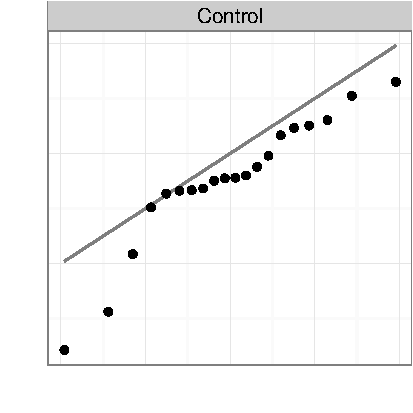
\includegraphics[width=0.22\textwidth]{figures/qqplots-1}
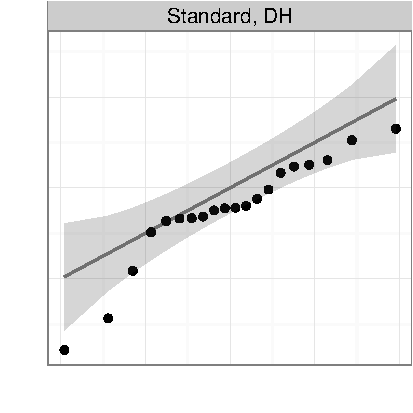
\includegraphics[width=0.22\textwidth]{figures/qqplots-2}
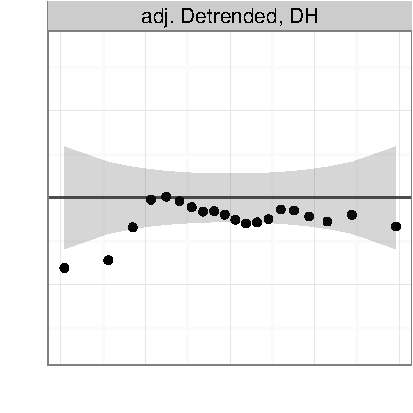
\includegraphics[width=0.22\textwidth]{figures/qqplots-3}
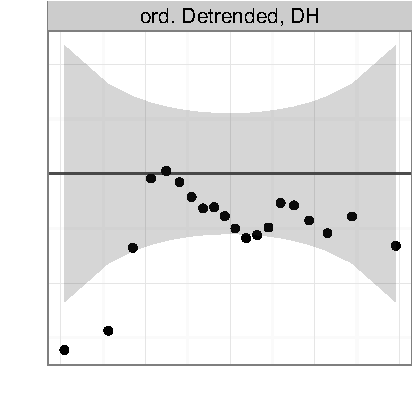
\includegraphics[width=0.22\textwidth]{figures/qqplots-4}

\includegraphics[width=0.22\textwidth]{figures/blank}
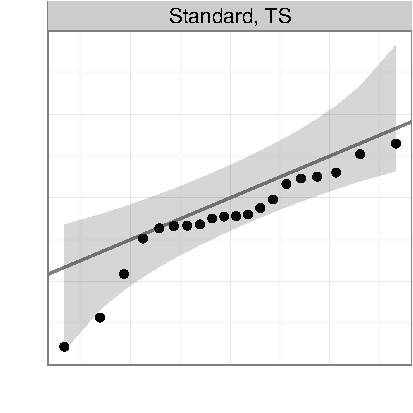
\includegraphics[width=0.22\textwidth]{figures/qqplots-5}
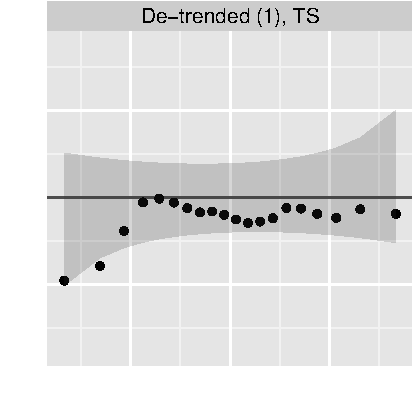
\includegraphics[width=0.22\textwidth]{figures/qqplots-6}
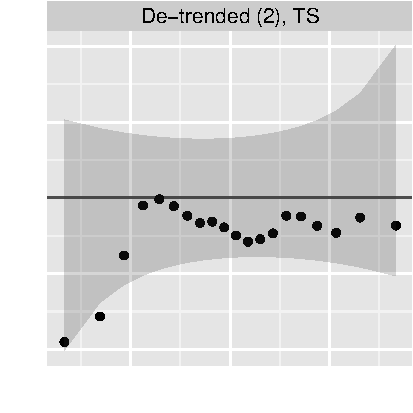
\includegraphics[width=0.22\textwidth]{figures/qqplots-7}
\caption{ \label{qqplots} \hh{Q-Q plot variations:} control, standard, and \hh{two versions of} de-trended \hh{Q-Q plots}, with Davison Hinkley (DH) or tail-sensitive (TS) 95\% confidence regions.}
\end{figure}
\afterpage{\clearpage}


In order to objectively evaluate  the three designs and quantify their effectiveness we make use of {\it lineup tests}.

\subsection{Lineup Tests}
Lineup tests have been introduced by \citet{buja:2009hp} to evaluate and quantify the significance of graphical findings. The idea behind a lineup test is that of a police lineup: the chart of the observed data is placed randomly among a set of so-called \emph{null charts}, showing data created consistently with the null hypothesis. In the setting of a lineup of normal Q-Q plots, the null hypothesis  is either that $F$ is standard normal or that $F$ is normal with parameters based on sample mean and variance.
If the `suspect'---i.e., the plot of the observed data---can be identified from the null charts, this counts as evidence against the null hypothesis. Multiple identifications of the data by independent observers then lead to a rejection of the null hypothesis. 
The lineup protocol also allows for an assessment of the power of a lineup \citep{mahbub:2013},  
%as the probability that in $N$ independent evaluations observers 
and by showing different renderings of the same data in lineups we can evaluate the power  of different designs \citep{Hofmann:2012ts}.

In considering the power of a lineup, we need to estimate the probability, $p_i$, that observer $i$ identifies the data from the lineup. If the observer is just guessing, this probability is $1/m$, where $m$ is the number of plots in the lineup.
The power of a lineup is then given as the probability to reject the null hypothesis. Let $Y$ be the number of identifications of the data plot in $N$ independent evaluations, and let $Y \sim F_N$. The power of the lineup is then the probability that more than $y_\alpha$ out of $N$ observers
choose the true plot, or more formally
\begin{equation}\label{eqn:power}
\widehat{\text{Power}} = \text{Power}_{N} = 1 - F_{Y} (y_{\alpha}),
\end{equation}
where $y_\alpha$ is the critical value for a given significance level $\alpha$, i.e.~$P(Y >  y_{\alpha}) \le \alpha$. $Y$ is composed of the sum of $N$ observers' (binary) decisions $Y_i \sim B_{1, p_i}$, where  $p_i$ is the probability that individual $i$ chooses the data plot. This probability  depends both on the strength of the signal in the data plot and an individual's visual ability.
Assessing this ability requires that each individual evaluates multiple lineups. 
If that is not possible, we must assume that all participants share the same ability, $p$. %, and the power calculation in Equation~\ref{eqn:power} simplifies to $1 - B_{N, \hat{p}}(x_\alpha)$, where $\widehat{p}$ is an estimate for the probability of choosing the data plot for a specific lineup.
Similar to classical inference, we can make use of power to assess the sensitivity of tests. This allows us to make decisions about designs for particular tasks by evaluating lineups displaying  the same data in different types of displays \citep{Hofmann:2012ts}. 

In the next section, we describe the simulation study used to compare the three \al{(four??)} Q-Q plot designs, and an initial comparison of the three designs is given. 
\al{In Section~\ref{sec:power2} we compare the power of the lineup test of normality to the classical normality tests. We use a generalized linear mixed model to compare the power of the three designs in Section~\ref{sec:power1}, and also explore the feedback of the independent observers to compare the rationale for plot selection (i.e., rejection of normality). We conclude with a discussion and outline areas for future research.}
% We use a generalized linear mixed model to compare the power of the three designs in Section~\ref{sec:power1}, and also explore the feedback of the independent observers to compare the rationale for plot selection (i.e., rejection of normality). Finally, we compare the power of a lineup test of normality to the classical normality tests in Section~\ref{sec:power2}, and outline areas for future research in Section~\ref{sec:discussion}. 


%------------------------------------------------------------------------------------
%------------------------------------------------------------------------------------

%------------------------------------------------------------------------------------
\section{Simulation Setup and Model}\label{sec:simu}
%------------------------------------------------------------------------------------

\hh{In order to evaluate the power of Q-Q plots and compare their performance to normal distribution tests, we make use of a simulation study, 
using samples of size $s \in \{20, 30, 50, 75\}$ from a $t_\nu$ distribution with $\nu \in \{2, 5, 10\}$ degrees of freedom. For each of these parameters we take two samples, resulting in a total of 24 samples.}
\alnote{I think using $n$ for sample size is most logical, though this does complicate the notation used in model (2).}

\hh{For the visual evaluation, we make use of Q-Q plots in a lineup test: each sample is randomly inserted among a set of 19 null plots constructed from samples of the same size drawn from the normal distribution. For each data \al{(XX observed (i.e., suspect) rather than data??)} sample, two sets of null plots are created, so that we have a total of 48 lineup samples. 
These lineup samples are rendered in each of the Q-Q plot variations, resulting in $48 \times 7 = 336$ different lineups.  Additionally, standard plots (both TS and DH bands) are rendered against $N(0, S^2)$ null data (see discussion below), adding another $2 \times 48 = 96$ lineups.
}


%To further develop the assessment of normality using lineups, we conducted a study comparing the three different versions of the Q-Q plot.
%We are testing three different versions of a Q-Q plot, 


%To investigate the power of the three different Q-Q plot versions, we sampled data from a $t$ distribution with varying degrees of freedom and sample sizes, and included a Q-Q plot of these data in a lineup of null charts drawn from standard normal samples of the same size.
For lineup tests it is extremely important to consider the generation of the null sets and the construction of the plots in the lineup. 
Null data sets must be created conistently with the null hypothesis. Here, we have two different null hypotheses to consider:

\begin{itemize}
\item{\bf Situation I:}
$H_0: F = N(0,1)$  \\
Null samples are drawn from a standard normal distribution; the reference line is the line of identity. Lines and envelopes are the same across all panels, in particular, all panels have the same scale. 
\item{\bf Situation II:} $H_0: F = N(0,S^2)$ \\
$S$ is based on the interquartile range of the data; null samples are drawn from $N(0, S^2)$. \\
The reference line has a slope of $S$ (and an intercept of 0).  All panels have the same scale. 
\end{itemize}

%\alnote{The generation of the null data makes sense to me, but is there a way to use bullet points on the right side of the table? That would help me read it...}

Examples for both \al{null} hypotheses are shown in Figure~\ref{fig:lps}. Both lineups show the same data set (in panel \#$(3^2-3)$\footnote{The little piece of calculus is imposing a small cognitive barrier that allows the reader to evaluate the lineup once without already being biased by knowing the location of the data panel.}). On the left the observed data stand out (all 33 observers picked the data plot); thus, we reject the null hypothesis of a standard normal distribution. On the right, the observed data do not stand out (only 3 out of 27 observers picked the data); thus, we do not reject the null hypothesis of a normal distribution with parameters $\mu=0$ and $\widehat{\sigma}=1.578$. 
\alnote{We need to straighten out our notation for the standard deviation. On this page we use both $\widehat{\sigma}$ and $\widehat{S}$.}

\begin{figure}[hbt]

\begin{subfigure}{0.5\textwidth}
\begin{knitrout}
\definecolor{shadecolor}{rgb}{0.969, 0.969, 0.969}\color{fgcolor}
\includegraphics[width=\maxwidth]{figure/unnamed-chunk-1-1} 

\end{knitrout}
\end{subfigure}
\begin{subfigure}{0.5\textwidth}
\begin{knitrout}
\definecolor{shadecolor}{rgb}{0.969, 0.969, 0.969}\color{fgcolor}
\includegraphics[width=\maxwidth]{figure/unnamed-chunk-2-1} 

\end{knitrout}
\end{subfigure}
\caption{\label{fig:lps} Lineup plots of standard Q-Q plots. The observed data is the same, but  reference lines and envelopes are based on a standard normal distribution on the left; while  reference lines and envelopes for the lineup on the right are based on a normal distribution $N(0, \widehat{S}^2)$, where $\widehat{S}$ is based on the IQR of the observed data.
The observed data plot in both lineups is displayed in panel \#$(3^2 - 3)$. }
\end{figure}
\afterpage{\clearpage}

Note that the above list of hypotheses is not exhaustive. Any theoretical distribution in a Q-Q plot corresponds to a  hypothesis test against that distribution, and as long as there is a method to generate samples under the null hypothesis, we do not even need to know the exact distribution. This allows us to assess situations in which we only have approximate or asymptotic results, which are otherwise hard, if not impossible, to investigate  with the (small) finite samples we typically deal with in practice.
\al{Additionally, we use the interquartile range (IQR) to estimate scale, as it is a standard practice for Q-Q plots.}
% The interquartile range (IQR) is used---as is standard practice for Q-Q plots---to estimate scale. 
Robust estimation of the variance is preferred for better assessment of the tails and outliers of the empirical distribution. We could use alternative estimators for variance, such as median absolute deviation (MAD) or adjusted MAD \citep{rousseeuw}, but this will likely also change the power of the corresponding lineup.

Using  Amazon MTurk \citep{amazon}, 1369 independent observers were recruited and asked to evaluate ten lineups each. \hh{Lineups were randomly assigned to participants, such that each participant
(i) evaluated each data set at most once, 
(ii) was exposed to multiple parameter settings (`harder' and `easier' lineups), and
(iii) evaluated each Q-Q plot design at most twice.

XXX discussion of amazon turk studies in comparison to lab experiments: practical considerations \citep{Kosara:2010}, study by \citet{cleveland:1984} re-run on Amazon MTurk with similar results by \citet{Heer:2010}.
}
%
Half of the lineups that observers were shown allowed for multiple choices of plots from a lineup for the final answer. Very few participants made use of this option. In the analysis we dealt with multiple answers to a lineup by using a weighting variable defined as the reciprocal of the number of answers given by a participant.





\begin{figure}[ht]
\centering
\begin{knitrout}
\definecolor{shadecolor}{rgb}{0.969, 0.969, 0.969}\color{fgcolor}
\includegraphics[width=\textwidth]{figure/compare-designs-1} 

\end{knitrout}
\caption{\label{fig:compare} \hh{Percentages of identifying the $t$ sample from lineups of different variations of Q-Q plots. Each lineup is shown as a dot. Filled dots indicate a (visually) significant deviation from normality (as determined in the user experiment). Dots of the same lineup data (sample and null data) are connected by a line.
The four lines in each panel correspond to four different lineups: the lines of the same color correspond to the same $t$-sample, but different null data; the lines of the other colour change both in sample and null data. The results are facetted by parameter setting: sample sizes $s$ (columns) vary from 20 to 75, degrees of freedom $\nu$ are shown in rows. With increasing sample size and decreasing degrees of freedom the percentage of picking the $t$ sample  from the normal samples generally increases. }
 }
\end{figure}
\afterpage{\clearpage}
\alnote{If we change the notation for the sample size, we will have to make changes in Figure 3.}
\alnote{The color in Figure 3 is lost in black and white printing. Should we pay for color in our submission? or should we add another aes parameter to ``double code''?}

Figure~\ref{fig:compare} shows percentages of data picks in the lineups under the different variations of Q-Q plots. 
\hh{All versions of Q-Q plots provide highly correlated results, and largely agree in the decision on normality. Filled circles indicate a  rejection of standard normality based on visual evaluation, open circles indicate a lack of rejection. Each of the panels shows the four lineups corresponding to the same sample size $n$ and degrees of freedom $\nu$ of the $t$ distribution.
Each line connects the evaluations based on the same lineup data (same data, same null plots).
Lines of the same color correspond to lineups with the same data sample, while differently colored lines show lineups of different samples.  Generally, within each panel, lines of the same color (lineups share the same data sample, but have different nulls) are closer together than lines of different color (different sample, different nulls).  }
As expected, the task of identifying non-normality becomes easier with increased sample size and more pronounced deviations from normality due to lower degrees of freedom. 
%All three versions provide highly correlated results, and largely agree for extreme decisions (all correct/all wrong evaluations). In the middle range de-trended Q-Q plots perform  worse than either standard or control Q-Q plots. 

\hh{Lineups of data samples from a $t_2$-distribution (bottom row)  are  rejected in lineups under all designs (with one exception), while the $t_{10}$ samples largely go undetected except for two of the larger samples.} 
Lineups of samples from a $t_5$ distribution \hh{show the most variability. Table~\ref{tab:no1} gives an overview of the number of rejections of a standard normal distribution by design. A more thorough discussion on the power of different designs follows in the next section.} 
 
\begin{table} 
\caption{\label{tab:no1} Number of rejections (out of 48) of standard normality by design.}
\centering
\begin{tabular}{lC{.6cm}C{.6cm}C{.6cm}C{.6cm}C{.6cm}C{.6cm}c}\hline
\bf Design & \multicolumn{2}{c}{\bf Standard} & \multicolumn{2}{c}{\bf De-trended (1)} & \multicolumn{2}{c}{\bf Detrended (2)} & \bf Control \\
\bf Confidence & DH & TS & DH & TS & DH & TS & --- \\ \hline \hline
Reject $N(0,1)$ & 29 & 30 & 30 & 32 & 26 & 28 & 28 \\ \hline
\end{tabular}
\end{table}
\afterpage{\clearpage}

% <<tab:n01, echo=FALSE, results='asis'>>=
% dt <- xtabs(~CIdesign + signif, data=dataset)
% @
%                signif
% CIdesign        FALSE TRUE
%   Standard.HD      18   30
%   Standard.TS      18   30
%   Detrended2.HD    18   30
%   Detrended2.TS    15   33
%   Detrended.HD     22   26
%   Detrended.TS     19   29
%   Control.HD       20   28






%------------------------------------------------------------------------------------
\section{Power: visual vs. classical}\label{sec:power2}
%-----------------------------------------------------------------------------------

It is important to recall that none of the data plots in the lineups were actually created using data from a normal distribution. Ideally, this should lead to rejection of the null hypothesis in every instance.
This is not quite true, as can be seen in Table~\ref{tab:reject} \al{XXX do we need to say more about the Table here?}, but what becomes evident is the high power  of visual inference. Using lineups we are able to reject non-normality much more often than with any of the classical tests.
% <<t15, echo=F>>= 
% if (!file.exists("data/turk15-summary.csv")) {
%   answers <- strsplit(as.character(t15$response_no), split=",")
%   t15$correct <- unlist(llply(1:length(answers), function(i) t15$obs_plot_location[i] %in% answers[[i]]))
%   t15$num_answers <- unlist(llply(answers, length))
%   
%   dsets2 <- ddply(t15, .(treatment, param_value, replicate), summarise, correct=sum(correct), evals=sum(num_answers))
%   require(vinference)
%   
%   dsets2$pvals <- unlist(llply(1:nrow(dsets2), function(i) {
%     correct <- floor(dsets2$correct[i])
%     n <- dsets2$evals[i]
%     vinference:::dvisual(x=correct, K=n, N=50000, m=20)$scenario3
%   }))
%   dsets2$signif <- dsets2$pvals < 0.05
%   write.csv(dsets2, file="data/turk15-summary.csv", row.names=FALSE)
% }
% dsets2 <- read.csv("data/turk15-summary.csv")
% @
% 
% <<t17, echo=F>>=
% if (!file.exists("data/turk17-summary.csv")) {
%   t0s <- read.csv("data/turk17-n0s.csv")
%   answers <- strsplit(as.character(t0s$response_no), split=",")
%   t0s$correct <- unlist(llply(1:length(answers), function(i) t0s$obs_plot_location[i] %in% answers[[i]]))
%   t0s$num_answers <- unlist(llply(answers, length))
%   
%   dsets <- ddply(t0s, .(design, param_value, rep), summarise, correct=sum(correct), evals=sum(num_answers))
%   require(vinference)
%   
%   dsets$pvals <- unlist(llply(1:nrow(dsets), function(i) {
%     correct <- floor(dsets$correct[i])
%     n <- dsets$evals[i]
%     vinference:::dvisual(x=correct, K=n, N=50000, m=20)$scenario3
%   }))
%   dsets$signif <- dsets$pvals < 0.05
%   write.csv(dsets, file="data/turk17-summary.csv", row.names=FALSE)
% }
% dsets <- read.csv("data/turk17-summary.csv")
% @
% 
% <<tab-rejects, echo=FALSE>>=
% dsets2$design <- "std_dh_lineup"
% dsets2$rep <- dsets2$replicate
% dsets <- rbind(dsets, dsets2[,names(dsets)])
% xtabs(data=dsets, ~design+signif)[2:3,2]
% dcast(data=dsets, param_value+rep~design, value.var="pvals")
% @
% 
% latex table generated in R 3.0.1 by xtable 1.7-1 package
% Mon May 27 20:57:50 2013
\begin{table}[ht]
\centering
\caption{\label{tab:reject}
 From left to right, we see the number of rejections from visual inference as well as the  Shapiro-Wilk, Anderson-Darling, Lilliefors,  Kolmogorov-Smirnov, and Cram\'er-von Mises tests for normality. Out of the 24 non-normal samples, 14 get rejected at the 5\% significance level based on evaluation by observers in the standard lineup with Davison-Hinkley confidence bands, 17 get rejected using lineups of standard Q-Q plots with TS confidence bands. None of the standard normal tests come close to those rejection rates. The power we observe here matches the power discussion by \citet{razali:2011} for the SW, AD, and the LF  tests. }

\begin{tabular}{rrrrrrrrr}
  \hline
 & \bf  Standard (TS/DH) & \bf SW & \bf AD & \bf LF   & \bf CvM & \\ 
  \hline
  \hline
%  reject $N(0,1)$ & 15 & 14 & 12  &   &  &   &  & 2\\ 
%  not reject & 19 & 20 & 22 &  &   &  &   & 44\\ 
%   \hline
  reject $N(0,S^2)$  & 17 / 14 &  8  & 5  &  5  & 4 & \\ 
%  not reject &  &  &  & 32 & 38  & 38 &  40 & \\ 
\hline
\end{tabular}
\end{table}
\afterpage{\clearpage}

\begin{figure}
\centering
\begin{knitrout}
\definecolor{shadecolor}{rgb}{0.969, 0.969, 0.969}\color{fgcolor}
\includegraphics[width=\maxwidth]{figure/unnamed-chunk-3-1} 

\end{knitrout}
\caption{\label{fig:pvals} \hh{ Comparison of visual tests and common normality tests. Each panel shows $p$-values  for each of  the two samples of size $n$ drawn from a $t_\nu$ distribution. If normality of a sample is rejected by a test, the point is hollow. Filled points indicate significant deviation from $N(0, s^2)$. Visual tests (shaded grey background) are generally  more powerful than common normality tests.} }
\end{figure}
\afterpage{\clearpage}
Figure~\ref{fig:pvals} shows an overview of the 24 samples' $p$-values  from the normal tests and estimated visual $p$-values from the lineups of Q-Q plots in the standard designs with either the Davison-Hinkley (DH) or the Tail-sensitive (TS) confidence bands. Out of the 24 samples the tests agree on ten samples, of which only three are rejected by every test.
%Figure~\ref{fig:visnorm} shows a scatterplot of $p$-values from the SW test and estimated $p$-values from the lineup of Q-Q plots in the standard design. Out of the 24 samples, the tests agree on 18, of which seven are rejections. Of the remaining six, five are rejected only by the visual test, and one is rejected by SW, but not by the visual test. Two samples on which the tests disagree are circled in figure~\ref{fig:visnorm}. The two lineups corresponding to these observations are shown in figure~\ref{fig:lpnorm}. The lineup on the left corresponds to a sample that is rejected by the SW test, but is not rejected by the visual test: only 1.5 decisions (at least one observer picked two panels in his/her response) out of 38 identified the data panel as the most different, which is not enough to reject the null hypothesis of $N(0, S^2)$. 
Figure~\ref{fig:lpnorm} shows two lineups for samples where the Shapiro-Wilk test and the visual test (using DH confidence bands) disagree. 
The lineup on the left corresponds to a $t_5$ sample of size $n = 30$ that is rejected by the SW test, but is not rejected by the visual test: only 1.5 decisions (at least one observer picked two panels in his/her response) out of 38 identified the data panel (in panel \#$(4^2-1)$) as the most different, which is not enough to reject the null hypothesis of $N(0, S^2)$. 
In contrast, the  lineup  on the right includes a $t_5$ sample of size $n=20$ (in panel \#$(3^2-1)$), which is picked by 23 out of 26 independent observers, leading to a very clear rejection of normality. 
The corresponding $p$-value in the SW test is 0.2318, after LF (0.1689) the test with the lowest $p$-value on this data sample out of all the normality tests.


The difference in significance between normality tests and the visual test might be due to the way the theoretical distribution against which the sample is compared is chosen. The normality tests are based on the sample mean and sample variance, both of which are affected by outliers. Compared to a normal distribution, the samples from a $t$ distribution exhibit heavier tails, and, in a finite sample, the heavier tails might look like outliers. By taking these outliers into account, the normality tests lose substantial power. The Q-Q plots, on the other hand, are based on a robust estimate of the scale based on the middle half of the empirical distribution. Q-Q plots are, therefore, less affected by outliers and the tails of a $t$ distribution are more easily distinguishable from the tails of a normal distribution, as can be seen in the lineup on the right of Figure~\ref{fig:lpnorm}. Compare this to the lineup in Figure~\ref{fig:lp3}, which is based on the same data, but the nulls are sampled from a normal distribution with a variance estimated as the sample variance. The data plot does not stand out, so we would not reject the null hypothesis based on this lineup. 
An inferior performance of normality tests based on the sample mean and variance is also observed by \cite{buja:2013} in the discussion of the TS test. 

\hh{XXX should we include a start on the comparison between TS and DH performance? TS is never not significant, if any other test is significant. }
% \begin{figure}
% \centering
% 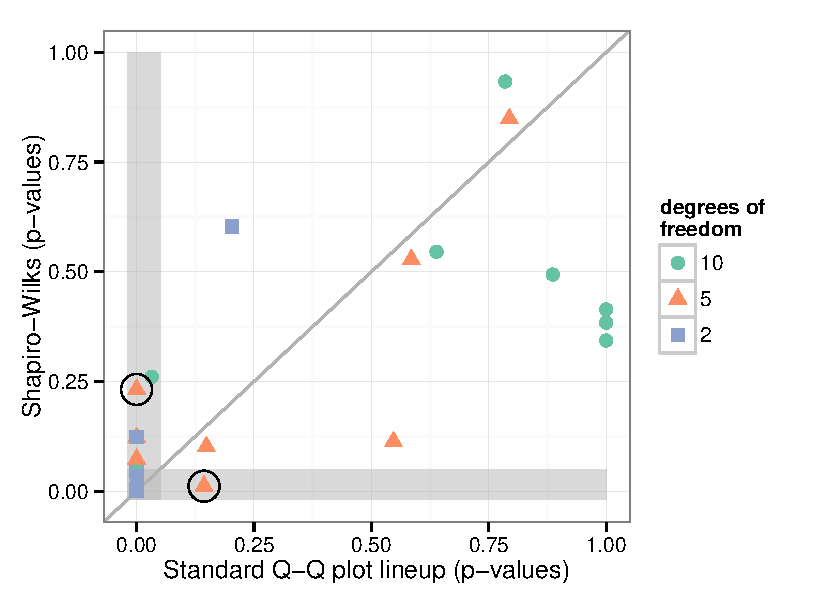
\includegraphics[width=0.5\textwidth]{figures/figvisnorm.pdf} 
% \caption{\label{fig:visnorm}  Scatterplot of $p$-values from the Shapiro-Wilk test and estimated $p$-values from lineups of Standard Q-Q plots. The grey shaded areas represent areas of rejection under at least one of the tests. The circled observations correspond to samples that lead to decidedly different decisions under the two tests. The lineups corresponding to these observations are shown in figure~\ref{fig:lpnorm}.}
% \end{figure}
% \afterpage{\clearpage}

\begin{figure}
\begin{subfigure}[t]{.49\textwidth}
\caption{Lineup of $t_5$ sample of size 30; data panel is panel \#$(4^2-1)$.}

\includegraphics[width=\maxwidth]{figure/plot-1} 

% \hfill
% %
% \begin{tabular}{C{0.75cm}|C{0.75cm}|C{0.75cm}|C{0.75cm}|c}
%  <<t1, dependson='plot1', results='asis', echo=FALSE>>=
% print(xtable(t(dx1)), floating=FALSE, only.contents=TRUE, include.rownames=FALSE, include.colnames=FALSE, zero.print="\\phantom{0.00}",  sanitize.text.function = function(x){x}, hline.after=1:3)
% @
% \end{tabular}
% \hfill

\end{subfigure}
\begin{subfigure}[t]{.49\textwidth}
\caption{Lineup of $t_5$ sample of size 20; data panel is panel \#$(3^2-1)$.}

\includegraphics[width=\maxwidth]{figure/plot2-1} 

% \hfill
% %
% \begin{tabular}{C{0.75cm}|C{0.75cm}|C{0.75cm}|C{0.75cm}|c}
%  <<t2, dependson='plot2', results='asis', echo=FALSE>>=
% print(xtable(t(dx2)), floating=FALSE, only.contents=TRUE, include.rownames=FALSE, include.colnames=FALSE, zero.print="\\phantom{0.00}",  sanitize.text.function = function(x){x}, hline.after=1:3)
% @
% \end{tabular}
% \hfill

\end{subfigure}
\caption{\label{fig:lpnorm}  \hh{On the left, visual inspection does not imply  a significant deviation of the sample from a normal distribution. On the right the deviation is highly significant.} \hh{The numbers in the bottom right of each panel show the number of times each was picked as the most different. } %The tables below the lineups show the number of times each of the panels was picked as the most different. 
Non-integer numbers result from multiple choice answers. %\hh{XXX} The italicized numbers refer to the panel that contains the actual sample.
}
\end{figure}
\afterpage{\clearpage}

\begin{figure}
\centering
\begin{knitrout}
\definecolor{shadecolor}{rgb}{0.969, 0.969, 0.969}\color{fgcolor}
\includegraphics[width=0.5\textwidth]{figure/lp3-1} 

\end{knitrout}
\caption{\label{fig:lp3} Lineup of standard design Q-Q plots showing the data of the lineup on the right in Figure~\ref{fig:lpnorm}. The hypothesized distribution is $N(0, \widehat{\sigma}^2)$, where $\widehat{\sigma}^2$ is estimated as the regular (i.e.~non-robust) sample variance, and nulls are drawn from that distribution. While not actually user tested, we do not think that the data stands out from the lineup.}
\end{figure}
\afterpage{\clearpage}
%-----------------------------------------------------------------------------------

%------------------------------------------------------------------------------------
\section{Power: three different designs of Q-Q plots}\label{sec:power1}
%-----------------------------------------------------------------------------------

\hh{In this section, we are investigating the differences that we see in Figure~\ref{fig:compare} of evaluations of the same data between different designs in more detail. We first model the results, then we investigate differences based on participants' answers. }

\hh{The premise underlying our} evaluation of the different Q-Q plot designs is that if participants find it easier to identify the data plot in one lineup than in another lineup (given identical data underlying the lineups), the first lineup uses the better design.

Let $Y_i$ be the outcome of the $i$th evaluation. Then $Y_i$ is a Bernoulli variable, where $\pi_i$ denotes the probablity of identifying the data plot from the lineup; i.e.~$P(Y_i = 1) = \pi_i = E[Y_i]$.   
The probability of identifying the lineup is affected by several factors: (a) the strength of the signal, i.e.~degrees of freedom of the $t$ distribution, and the sample size, (b) a human factor, i.e~the visual ability of the observer, and (c)  the `lineup factor': depending on which $m-1$ representatives of the test distribution the null plots show, lineups of the same data plot can have different difficulty. We capture all of this in a logistic regression model with fixed effects for signal strength and random effects for lineup difficulty and user ability. More specifically: 

%Next, we model the aforementioned probability $p_i$ with which observer $i$ picks the true data from a lineup. 
%Let $X_i \sim B_{1, \pi_i}, 1 \le i \le n$, where $X_i$ is the binary decision on the $i$th evaluation and $\pi_i$ is the probability with which the observer chooses the data plot. This probability is influenced by a number of factors:

\begin{center}
\begin{tabular}{lp{5in}}
$\tau$ & the design used in the lineup; this is either {\it Control} or one of  {\it \{  Standard, De-trended (1), De-trended (2)\}} in combination with a choice of confidence band (HD, TS), \\
&  the specific parameters under which the data for the lineup were created: \\
&  $\delta$ \ \ \ degrees of freedom (2, 5, 10) {of the $t$ distribution} and \\
&  $\nu$  \ \ \ sample size (20, 30, 50, 75), \\
$d$ &  the level of difficulty based on the actual sample, and \\
$u$ & the users' subjective abilities.
 \end{tabular}
\end{center}
%

\alnote{We need to think about the notation here.}
\begin{eqnarray} \label{eq:model}
g(\pi_i) &=& \eta_i = \mu + \tau_{j(i)} +\delta_{k(i)}+ \nu_{s(i)} + u_{u(i)} + d_{d(i)},\\ \nonumber
Y &=& g^{-1}(\eta) + \varepsilon
\end{eqnarray}
where $g$ is the logit link function, and $j(.), k(.), s(.), u(.)$, and $d(.)$ are  indexing functions that relate evaluation $i$ to the corresponding levels in the factor variables, to the observer, or a particular data sample. More specifically, $j(i) \in \{$Control, Standard (DH), Standard (TS), De-trended (DH), De-trended (TS), De-trended2 (DH), De-trended2 (TS)$\}$; $k(i) \in \{2,5,10\}$; $s(i) \in \{20, 30, 50, 75\}$; $u(i)$ maps to the participant's id of the $i$th evaluation; and $d(i)$ identifies the particular sample \hh{and null data} used. 
Both user ability, $u$, and sample difficulty, $d$, are modeled as independent, normally distributed  random effects, i.e. $u_{u(i)} \sim N(0, \sigma_u^2)$, $d_{d(i)} \sim N(0,\sigma_d^2)$ with cov$(u, d) = 0$. We further assume that $E[\varepsilon] = 0$ and Var$[\varepsilon]=\sigma^2$.
%
\hh{Table~\ref{tab:coefs} gives an overview of the coefficients. As could be seen in various figures before, an increase in signal strength (larger sample size, fewer degrees of freedom) result in lineups, in which the sample is picked out more often by observers.}

\hh{Aside from that,} the design of the Q-Q plot is of huge importance for the probability of choosing the data plot: compared to the control chart, add-on confidence bands help with evaluation in the standard design, but the difference is not significant.  

\hh{The first de-trended version of Q-Q plots, in which the aspect ratio is kept the same as in the standard plot, shows significant increases in detecting non-normality. }
Surprisingly, the \hh{second version of} de-trended Q-Q plots is significantly less powerful in detecting non-normality. \hh{De-trended (2) Q-Q plots with DH bands are actually performing significantly worse than the control charts, while Q-Q plots with the TS bands just lose their previous gain from de-trending.} \hh{It seems that the additional space on the $y$-axis emphasizes artifacts that are hard to judge, because distances in the $x$ direction have a different meaning than distances in the $y$ direction. Due to the difference in aspect ratio plotted distances between points are not proportional to distances in the data space.} 

\hh{For the other two designs, Q-Q plots with TS bands have slightly less power than the same version of Q-Q plots with DH bands. While not significant, this makes sense, and is likely due to TS bands being wider in the center of the distribution and at the tips of the tails.}





% latex table generated in R 3.1.1 by xtable 1.7-3 package
% Sat Feb 21 18:16:18 2015
% cis <- data.frame(confint(m1, method="Wald"))
% names(cis) <- c("lower", "upper")
% cis$estimates <- fixef(m1)
% 
% #ciprofile <- data.frame(confint(m1))
% library(xtable)
% dc <- cis[,c("estimates", "lower", "upper")]
% dc$odds <- exp(dc$estimates)
% dc$odds.low <- exp(dc$lower)
% dc$odds.high <- exp(dc$upper)
% 
% print(xtable(dc))
\begin{table}[ht]
\caption{\label{tab:coefs} \hh{Linear estimates and corresponding odds based on Model (1).  95\% Wald confidence intervals are given in parentheses.}}
\centering
%\begin{tabular}{rr>{ (}r<{,}>r<{) }rrl}
\begin{tabular}{rr>{ (}r@{, }r<{) }rr>{ (}r@{, }r<{) }}
\cline{2-4}\cline{6-8}
& estimates & \bf low & \bf high && odds &  \bf low & \bf high \\ 
 \cline{2-4} \cline{6-8}
%  \hline
  Intercept & \bf -4.84 & \bf -6.19 & \bf -3.49 && \bf 0.01 & \bf 0.00 & \bf 0.03 \\ [3pt]
\multicolumn{1}{r}{\bf design (CI)} \\  
Control & 0.00 & \multicolumn{2}{c}{---} && 1.00 & \multicolumn{2}{c}{---}\\
Standard (DH) & 0.10 & -0.08 & 0.29 && 1.11 & 0.92 & 1.33 \\ 
  Standard (TS) & -0.18 & -0.40 & 0.04 && 0.83 & 0.67 & 1.04 \\ [2pt]
%
Detrended 1 (DH) & \bf 0.42 & \bf 0.20 & \bf 0.64 && \bf  1.52 & \bf 1.22 & \bf 1.89 \\ 
  Detrended 1 (TS) & \bf 0.32 & \bf 0.10 & \bf 0.53 && \bf 1.37 & \bf 1.10 & \bf 1.70 \\ [2pt]
%
Detrended 2 (DH) & \bf -0.42 & \bf -0.61 & \bf  -0.24 && \bf 0.66 & \bf 0.54 & \bf  0.79 \\ 
  Detrended 2 (TS) & 0.03 & -0.19 & 0.25 && 1.03 & 0.83 & 1.28 \\ [3pt]
\multicolumn{1}{r}{\bf sample size} \\  
20 & 0.00 & \multicolumn{2}{c}{---} && 1.00 & \multicolumn{2}{c}{---}\\
  30 & 1.07 & -0.45 & 2.60 && 2.92 & 0.64 & 13.43 \\ 
  50 & \bf 3.00 & \bf 1.47 & \bf 4.53 && \bf 20.13 & \bf 4.37 & \bf 92.77 \\ 
  75 & \bf 2.36 & \bf 0.83 & \bf 3.89 && \bf 10.59 & \bf 2.29 & \bf 49.04 \\ [3pt]
\multicolumn{1}{r}{\bf degrees of freedom} \\  
 2 & \bf 6.08 & \bf 4.74 & \bf 7.42 && \bf 436.30 & \bf  114.26 & \bf 1666.09 \\ 
 5 & \bf 2.35 & \bf 1.03 & \bf  3.66 && \bf 10.44 & \bf 2.80 & \bf 38.93 \\ 
10 & 0.00 & \multicolumn{2}{c}{---} && 1.00 & \multicolumn{2}{c}{---}\\
\cline{2-4} \cline{6-8}
\end{tabular}
\end{table}
\afterpage{\clearpage}



% \begin{table}[ht]
% \centering
% \caption{\label{tab:reject1}
% %
%  From left to right, we see the number of rejections from different lineup designs.
%   Out of the 24 non-normal samples, 12 get rejected at the 5\% significance level based on evaluation of the de-trended design. Besides these 12 normality is rejected for another two samples by lineups in the control design. The standard design detects non-normality in yet another design. }
% 
% \begin{tabular}{rrrr}
%   \hline
%  & Standard & Control & De-trended  \\ 
%   \hline
%   \hline
%   reject $N(0,1)$ & 15 & 14 & 12    \\ 
% \end{tabular}
% \end{table}


%In terms of rejections of the null hypothesis, this means that normality is rejected in 24 out of the 48 lineups of the de-trended (2) Q-Q plot. All of these cases are being rejected in all of the other designs as well, but using the control design another four lineups reject normality, and the standard design rejects yet another lineup.

To further investigate the difference between the designs, consider figure \ref{fig:rotstd}. Here, we consider a sample from the $t_2$ distribution of size $n=20$ that is rejected \hh{from all designs besides the de-trended (2) Q-Q plots with a DH band.}  
\hh{The de-trended (2) DH band is shown on the left side of figure~\ref{fig:rotstd}. Instead of the data sample in panel \#$(2^2+1)$ observers pick panel \#7 in 32.2 out of 45 evaluations. For any of the other designs, as e.g.\ the de-trended (2) Q-Q plot with TS bands on the right of figure~\ref{fig:rotstd}, observers pick the panel of the data sample at a rate that leads to a rejection of normality.  }
%Instead of focusing on the panel showing the sample, observers focus on panel \#$(3^2-2)$ (with 18 out of 21 picks). This panel was picked as being most different 9 out of 27 times in the standard design, too, indicating that there is something special about it, but most observers (16 out of 27) picked the data in panel \#$(2^2+1)$ from the standard design. 
\begin{figure}[hbt]
%\begin{subfigure}{0.5\textwidth}

%\end{subfigure}
\begin{subfigure}{0.5\textwidth}
\begin{knitrout}
\definecolor{shadecolor}{rgb}{0.969, 0.969, 0.969}\color{fgcolor}
\includegraphics[width=\maxwidth]{figure/notrotated2-1} 

\end{knitrout}
\end{subfigure}
\begin{subfigure}{0.5\textwidth}
\begin{knitrout}
\definecolor{shadecolor}{rgb}{0.969, 0.969, 0.969}\color{fgcolor}
\includegraphics[width=\maxwidth]{figure/notrotated3-1} 

\end{knitrout}
\end{subfigure}
\caption{\label{fig:rotstd}Lineups of the same data in two different designs. %In the standard design the data sample (in panel \#$(2^2+1)$) is identified 16 out of 27 times, leading to a rejection of normality. 
In the lineup on the left the data sample in panel \#$(2^2+1)$ is only identified \hh{2.8 times in 45} evaluations in the lineup showing the de-trended (2) design \hh{with a DH band}. Observers instead pick panel \#$(3^2-2)$ \hh{32.2} times. \hh{The lineup on the right shows the same data in a de-trended (2) Q-Q plot design using the TS confidence band. The data sample is picked 7.2 times in 27 evaluations, leading to a rejection of normality at a 5\% signficance level.}}
\end{figure}
\afterpage{\clearpage}

%xtabs(weight~response, data=subset(turkw, data_name==frames[1] & plot_location==5 & treatment=="Standard"))
%xtabs(weight~response, data=subset(turkw, data_name==frames[1] & plot_location==5 & treatment=="Rotated"))
\hh{Only 6.3\% of all evaluations made use of the option of giving feedback for the reason of their choice in form of a free-form answer. }
%
\hh{The two participants who gave a free-form answer for their choice in the lineup on the left hand side of figure~\ref{fig:rotstd}, picked panel \#7 from the de-trended lineup, and stated that this panel was the one with the ``most dots outside the shaded area,'' i.e.~they focused on the middle of panel \#7}. 

\hh{XXX update March 17 XXX - there's nothing in the choices that participants gave. in the additional experiment participants only commented in about 1\% of the lineups on their reason. I think it'd be better to get rid of this argument. Instead, I've added all of the lineups, in which DH and TS result in different outcomes. XXXX}

This is not a singular occurrence---when investigating \hh{all lineups of the same design which lead to different outcomes depending on the choice of confidence band (an exhaustive list of all these lineups is given in the appendix in section~\ref{sec:lplist}), we find that for designs using DH bands, panels were picked in favor of the data sample, when dots were outside the shaded area. This happened both in the tails and in the middle part of the distribution.  } 
%overall reasoning we took a closer look at the effect of the  words ``area'' and ``outside'' in the reason participants gave for making their choice of plot %(figure~\ref{fig:rotfalse}). 
\hh{This is consistent with the findings in \citet{buja:2013}, which motivated the research into Tail-Sensitive confidence bands. These bands define a test of normality and are narrower in the tails (but skew) than those associated with the Kolmogorov-Smirnov test, while slightly more conservative in the middle of the distribution.}


%This is not a singular occurrence---when investigating  overall reasoning we took a closer look at the effect of the  words ``area'' and ``outside'' in the reason participants gave for making their choice of plot %(figure~\ref{fig:rotfalse}). 
%As expected, these words barely occur in the control design (where there is no shaded area).


%\hh{investigate whether outside area is also indicative for TS plots}
%It seems to help in identifying the data plot in the standard design, but it severely  increases the chance of picking a null plot in the de-trended design. Why is that? The de-trended version is making better use of the space in the plot, it therefore  emphasizes deviations of points from the $x$-axis (i.e.~the theoretical distribution) and with it  the fact whether individual points are inside or outside the shaded areas corresponding to the (pointwise) 95\% confidence intervals. The responses suggest that participants take the shading very seriously and make their choice dependent on it. It also seems that the confidence bands mislead people---this suggests, that for the de-trended Q-Q plot design we might have to re-think how to display confidence intervals: it might be better to  either use  a more conservative  confidence level or change the approach altogether from pointwise confidence intervals to simultaneous confidence bands as, for example, discussed by \citet{Rosenkrantz:2000fd}.
% \alnote{This would be a very natural place to put in TAS citations: Aldor-Noiman et al (2013) and Rosenkrantz (2000). }
% \hhnote{comment on Rosenkrantz is missing still}





% <<sentiment, echo=FALSE>>=
% library(wordcloud)
% library(tm)
% for (i in 1:nrow(design)) {
% words.corpus <- Corpus(DataframeSource(data.frame(design$otherw[i])))
% words.corpus <- tm_map(words.corpus, removePunctuation)
% 
% tdm <- TermDocumentMatrix(words.corpus)
% m <- as.matrix(tdm)
% v <- sort(rowSums(m),decreasing=TRUE)
% d <- data.frame(word = names(v),freq=v)
% pal <- brewer.pal(9, "BuGn")
% pal <- pal[-(1:2)]
% png(sprintf("wordcloud/wordcloud-%s-%s.png",design$CIdesign[i], design$choice[i]), width=960,height=600)
% wordcloud(d$word,d$freq, scale=c(8,.3),min.freq=2,max.words=100, random.order=T, rot.per=.15, colors="black", vfont=c("sans serif","plain"))
% dev.off()
% }
% @
% 
% % \begin{figure}[hbt]
% % \centering
%  <<rotfalse,echo=FALSE, fig.width=6, fig.height=6, out.width='.65\\textwidth'>>=
% qplot(CIdesign, fill=choice, weight=pct, data=subset(designm, CIdesign != "Control.HD"), position="fill") + scale_fill_brewer(palette="Set2") + facet_wrap(~variable) + theme_bw()
%  @
% % \caption{\label{fig:rotfalse}Mentioning ``outside'' or ``area'' in the reason for selecting the plot from the lineup increases the probability of not identifying the data plot by a large factor in de-trended Q-Q plots. }
% % \end{figure}
% % \afterpage{\clearpage}

\begin{figure}[hbt]
\centering
\begin{knitrout}
\definecolor{shadecolor}{rgb}{0.969, 0.969, 0.969}\color{fgcolor}
\includegraphics[width=0.7\textwidth]{figure/trtplot-1} 

\end{knitrout}
\caption{\label{fig:choices}Overview of reasons participants gave for  their answer. ``Outliers" as a reason drastically improves the chance of identifying the data plot. All the other reasons either have no effect or decrease the chance of picking the data. It is curious, that more observers gave ``left side different" as a reason than ``right side different";   all the samples  come from a  $t$-distribution, so deviations in the extremes should therefore also be symmetric.}
\end{figure}
\afterpage{\clearpage}

\hh{Figure~\ref{fig:choices} summarizes the reasons participants gave for the choice of plot they selected. Bars on the left show  identifications of the data plot, bars on the right represent selections of a null plot. The reasons represent the five reasons offered  to participants. Notably, the reasons do not seem to differentiate between the different designs. Stating ``outliers'' as a reason for choosing a plot is helpful across all designs in picking the data out of the lineup. Stating ``points are on a curve'' or ``other"  as the reason for choosing a plot decreases the chance for this plot to be the data plot. ``Right side different'' or ``left side different" do not seem to have much of an effect. } 
%is a big difference in the percentages of ``right'' and ``left.'' Participants favored to give ``left side different'' as a reason over ``right side different'', even though all distributions involved were symmetric, and therefore deviations from normality should also manifest themselves in a symmetric fashion.

%\hhnote{another idea: go through reasons for choices. For standard design the line was often interpreted as a line of fit (how often for the de-trended design?), ie. we are tapping into what general population knows about regression. While this is not completely appropriate, the knowledge transfer might be the reason for the better performance.}

%------------------------------------------------------------------------------------
\section{Discussion and Conclusion}\label{sec:discussion}
%-----------------------------------------------------------------------------------
In the comparison of the three designs of Q-Q plots, de-trended Q-Q plots turn out to have significantly less power in detecting non-normality than Q-Q plots in the standard and the control design. This is surprising, as results from cognitive psychology suggest that the de-trended version has superior qualities. From the additional reasoning provided by participants regarding their choice of plot it becomes obvious that this choice is mainly driven by points outside the shaded area depicting 95\% confidence intervals. This happens primarily in the middle of the distribution, confirming results by \citet{buja:2013}, and reopens the question of whether the design or the choice of confidence calculation is the reason for the inferiority. It would also make sense to fix the aspect ratio of plots in the de-trended design to make comparisons between the range of points in both axis directions possible.
All versions of Q-Q plots under consideration here are significantly better at detecting deviations from normality than classical normality tests. A contributing factor to this superior power might be  that in  Q-Q plots the whole sample is assessed rather than being reduced to the single value considered for the test statistic. 
Contributing to the power is also the robust estimation of the parameters for the normal distribution drawn as a line of fit in  Q-Q plots, while most normality tests are based on the outlier sensitive sample variance. %$S^2 = \sum_i(x_i - \bar{X})^2/(n-1)$ 
This is consistent with findings in \citet{buja:2013} and  also poses the question of whether the power of classical normality tests might  be improved by using robust estimates for the mean and variance of the sample.

Q-Q plots are not restricted to the assessment of normality. In fact, they provide a general framework for testing any distributional assumptions. Used in the setting of lineups, they in particular allow an assessment of limiting distributions, i.e.~for example, lineups allow us to investigate distributions of
 samples from approximate normal or asymptotic normal distributions, for which  there exists  no classical test for finite sample sizes, whereas the lineup protocol provides us with a valid testing system
  as long as there is a method  to generate data under the null hypothesis for creating null plots in the lineup.
 

One of the drawbacks of the lineup test framework is that it comes at a higher cost, both monetary and in time, than classical testing.
However, developments such as {\tt nullabor} \citep{nullabor} or {\tt vis.test} \citep{vistest} allow us to be, at least to a degree, our own testers. For tests that are of a more sensitive nature, the cost of a test using a crowd-sourcing service is certainly a small enough item in the overall project budget that it is a feasible 
option. It also discourages the analyst from multiple testing!

Several possibilities for immediate extensions are obvious: the simulation study here is only concerned with deviations from normality as given by the $t$-distribution. Other types of deviations, such as skewed distributions or mixture distributions, would be interesting to consider as well. We doubt that the overall results would change dramatically, but it might provide more insight into what observers consider in making their assessments. 
The application of the lineup framework based on the related probability (P-P) plots poses a natural next question: \citet{koehler91} comment on the higher sensitivity of  P-P plots  to discrepancies in the middle of the distribution, such as caused by multiple modes. We can verify this and other statements for large samples and based on distributions. Lineups allow us to quantify the extent to which these statements hold for small sample sizes.


\bibliographystyle{asa}
\bibliography{qqplots}

\newpage
\begin{appendix}
\section{Model and Results}

%Next, we model the aforementioned probability $p_i$ with which observer $i$ picks the true data from a lineup. 
%Let $X_i \sim B_{1, \pi_i}, 1 \le i \le n$, where $X_i$ is the binary decision on the $i$th evaluation and $\pi_i$ is the probability with which the observer chooses the data plot. This probability is influenced by a number of factors:

% \begin{center}
% \begin{tabular}{lp{5in}}
% $\tau$ & the combination of design used in the lineup  \{ Control, Standard, De-trended (1), De-trended (2)\} and confidence interval (HD, TS), \\
% &  the specific parameters under which the data for the lineup were created: \\
% &  $\delta$ \ \ \ degrees of freedom (2, 5, 10) {of the $t$ distribution} and \\
% &  $\nu$  \ \ \ sample size (20, 30, 50, 75), \\
% $d$ &  the level of difficulty based on the actual sample, and \\
% $u$ & the users' subjective abilities.
%  \end{tabular}
% \end{center}
% %
% 
% %



% latex table generated in R 3.1.0 by xtable 1.7-3 package
% Sun Aug  3 11:20:58 2014
% xtable(summary(m1)$coefficients, digits=c(0,2,3,2,4))
\begin{table}[ht]
\centering
\caption{\label{tab:model} Coefficients and significances corresponding to  model (\ref{eq:model}). The type of design is important for the power of a lineup. \hh{ De-trended (2) Q-Q plots with Davison-Hinkley confidence bands lose a significant amount of power compared to the other  versions of Q-Q plots. If TS intervals are used, this loss does not occur. De-trended (1) Q-Q plots with fixed aspect ratio perform significantly better than all of the other versions of Q-Q plots.}}
\begin{tabular}{rrrrrl}
   \hline
  &\bf Estimate &\bf Std. Error &\bf z value &\bf Pr($>$$|$z$|$) & \\ 
   \hline
    Intercept & -4.84 & 0.690 & -7.02 & 0.0000 & ***\\ 
 \multicolumn{3}{l}{\bf design (CI)} \\
   Control & 0.00 & ----- & ----- & ----- \\ [2pt]
   Standard (DH) & 0.10 & 0.093 & 1.12 & 0.2618 \\ 
   Standard (TS) & -0.18 & 0.113 & -1.62 & 0.1053 \\ [2pt]
   Detrended (DH) & 0.42 & 0.111 & 3.77 & 0.0002 & ***\\ 
   Detrended (TS) & 0.32 & 0.111 & 2.85 & 0.0044 & **\\ [2pt]
   Detrended 2 (DH) & -0.42 & 0.094 & -4.49 & 0.0000 & ***\\ 
   Detrended 2 (TS) & 0.03 & 0.112 & 0.27 & 0.7846 \\ [3pt]
 \multicolumn{3}{l}{\bf sample size} \\
   20 & 0.00 & ----- & ----- & ----- \\ 
   30 & 1.07 & 0.778 & 1.38 & 0.1678 \\ 
   50 & 3.00 & 0.780 & 3.85 & 0.0001 & ***\\ 
   75 & 2.36 & 0.782 & 3.02 & 0.0026 & **\\ [3pt]
 \multicolumn{3}{l}{\bf degrees of freedom} \\
  2 & 6.08 & 0.684 & 8.89 & 0.0000 & ***\\ 
  5 & 2.35 & 0.671 & 3.49 & 0.0005 & ***\\ 
  10 & 0.00 & ----- & ----- & ----- \\ 
    \hline
\multicolumn{6}{l}{Signif. codes:  0 $\le$ *** $\le$ 0.001 $\le$ ** $\le$ 0.01 $\le$ * $\le$ 0.05 $\le$ . $\le$ 0.1 $\le$ ' ' $\le$ 1}
\end{tabular}
\end{table}
\afterpage{\clearpage}

Table~\ref{tab:model} gives an overview of the estimated coefficients for model (\ref{eq:model}). 
Estimates of the variance components are $\widehat{\sigma}_u = 0.66$, $\widehat{\sigma}_d=1.87$, and $\widehat{\sigma} = 0.3$. Variances of user ability and data difficulty are large relative to residual variance, indicating that both random effects are necessary.
%
%Figure~\ref{fig:ranef} shows histograms of the predicted random effects for participants' abilities (left) and difficulty level of lineups (right). 
Compared to the difficulty level of lineups, participants' abilities only vary little. The difference between best and worst performance by participants has an effect of at most an estimated 
3.2-fold probability of detecting the data plot from a lineup. 

\section{Differences between Davison-Hinkley and Tail-sensitive confidence bands}\label{sec:lplist}

%
In this section we are listing all lineups in which lineups of Q-Q plots with a  Davison-Hinkley band results in a different outcome than the same Q-Q plot design with a TS band. 
Under the standard design there is one lineup, the detrended (1)  design has two lineups with different outcomes, while the detrended (2) design has four lineups with different outcomes. They are shown in figures~\ref{fig:lpsstds},~\ref{fig:lpsdt1}, and~\ref{fig:lpsdt2}, respectively. 

\begin{figure}
\centering
\begin{knitrout}
\definecolor{shadecolor}{rgb}{0.969, 0.969, 0.969}\color{fgcolor}
\includegraphics[width=0.4\textwidth]{figure/lpsstds-1} 
\includegraphics[width=0.4\textwidth]{figure/lpsstds-2} 

\end{knitrout}
\caption{\label{fig:lpsstds} Standard lineups with different outcomes depending which confidence band is used. The outlined panel marks the location of the data sample, the numbers at the bottom right are showing the number of votes each of the panels was picked by observers.  }
\end{figure}
\afterpage{\clearpage}


\begin{figure}
\centering
\begin{knitrout}
\definecolor{shadecolor}{rgb}{0.969, 0.969, 0.969}\color{fgcolor}
\includegraphics[width=0.4\textwidth]{figure/lpsdt1-1} 
\includegraphics[width=0.4\textwidth]{figure/lpsdt1-2} 
\includegraphics[width=0.4\textwidth]{figure/lpsdt1-3} 
\includegraphics[width=0.4\textwidth]{figure/lpsdt1-4} 

\end{knitrout}
\caption{\label{fig:lpsdt1} De-trended (1) lineup with different outcomes depending on the choice of confidence band. The outlined panel marks the location of the data sample, the numbers at the bottom right are showing the number of votes each of the panels was picked by observers.  }
\end{figure}
\afterpage{\clearpage}



\begin{figure}
\centering
\begin{knitrout}
\definecolor{shadecolor}{rgb}{0.969, 0.969, 0.969}\color{fgcolor}
\includegraphics[width=0.4\textwidth]{figure/lpsdt2-1} 
\includegraphics[width=0.4\textwidth]{figure/lpsdt2-2} 
\includegraphics[width=0.4\textwidth]{figure/lpsdt2-3} 
\includegraphics[width=0.4\textwidth]{figure/lpsdt2-4} 
\includegraphics[width=0.4\textwidth]{figure/lpsdt2-5} 
\includegraphics[width=0.4\textwidth]{figure/lpsdt2-6} 

\end{knitrout}
\caption{\label{fig:lpsdt2} Three of the  four sets of de-trended (2) lineups with different outcomes depending which confidence band is used. The outlined panel marks the  location of the data sample, the numbers at the bottom right are showing the number of votes each of the panels was picked by observers. The fourth set of lineup with a different outcome is shown in figure~\ref{fig:rotstd}. }
\end{figure}
\afterpage{\clearpage}







% 
% \section{Demographics and other study results}
% %-----------------------------------------------------------------------------------
% 
% <<attempts, echo=FALSE, dependson='data'>>=
% suppressMessages(require(Hmisc))
% attempts <- ddply(turkw, .(attempt), summarise, 
%                   cmean=wtd.mean(correct, weights=weight, na.rm=TRUE),
%                   csd=sqrt(wtd.var(correct, weights=weight, na.rm=TRUE)/sum(weight)),
%                   tt=wtd.mean(time_taken, weights=weight, na.rm=TRUE),        
%                   sdtt=sqrt(wtd.var(time_taken, weights=weight, na.rm=TRUE)/sum(weight)),
%                   nevals=sum(weight)
%                   )
% @
% 
%  Similar to observations made in other lineup experiments \citep{Majumder:2014up}, there is no indication of a ``learning'' effect within a participant's first ten answers (see figure~\ref{fig:attempts}), indicating that lineups make use of an observer's inherent ability rather than a learned skill. The overall proportion of correct responses is very stable, fluctuating around round(with(turkw, Hmisc::wtd.mean(correct, weights=weight)),2) with a standard deviation of about round(mean(attempts$csd),2).  What does change with the number of attempts is the time taken by participants to answer a lineup. From initially round(attempts$tt[1],1) seconds in the first answer, the response time drops to round(attempts$tt[10],1) seconds at the tenth evaluation.
% \begin{figure}
% \centering
% \begin{subfigure}[b]{.35\textwidth}
% <<fig1, echo=FALSE, dependson='attempts', fig.width=4, fig.height=4>>=
% qplot(attempt, cmean, data=subset(attempts, attempt <= 10)) + 
%   ylim(c(0,1)) + 
%   scale_x_discrete(breaks=1:10) + 
%   geom_segment(aes(x=attempt, xend=attempt, y=cmean+1.96*csd, yend=cmean-1.96*csd, group=attempt)) +
%   ylab("Proportion of correct responses") + theme_bw()
% @
% \end{subfigure}
% \begin{subfigure}[b]{.35\textwidth}
% <<fig2, echo=FALSE, dependson='attempts', fig.width=4, fig.height=4>>=
% qplot(attempt, tt, data=subset(attempts, attempt <= 10)) + 
%   ylim(c(0,60)) + 
%   scale_x_discrete(breaks=1:10) + 
%   geom_segment(aes(x=attempt, xend=attempt, y=tt+1.96*sdtt, yend=tt-1.96*sdtt, group=attempt)) +
%   ylab("Response time in seconds") + theme_bw()
% @
% \end{subfigure}
% \caption{\label{fig:attempts}Proportion of correct answers by attempt (left) and time taken in each of the first ten attempts (right). The proportion of correct responses stays constantfor successive attempts, while the time to answer decreases significantly over the same number of attempts.}
% \end{figure}
% 
% \hhnote{gender, education, geographic location?}
\end{appendix}

\end{document}
